\section{Nõuete defineerimine}
\label{chapters:analysis_requirements}
\subsection{Funktsionaalsed nõuded}
\label{subsec_func_req}
Funktsionaalsete nõuete määramisel lähtutakse erinevate osapoolte vajadusest - süsteemi kasutaja ja süsteemi 
administraator. Kavandatav funktsionaalsus on määratud lähtuvalt peatükis \ref{chapters:problem_statement_existing_solutions} toodud
eksisteerivate lahenduste uurimisest.

Infosüsteemi kasutaja (klient) peab saama teostada peatükis \ref{chapters:problem_statement_research} toodud ehituskonstruktsiooni niiskustehnilise toimivuse analüüsi,
kasutades andmebaasis olevad ehitusmaterjalid. Ehitusmaterjalid võivad olla andmebaasisse lisatud administraatori poolt (avalikud materjalid, mida kõik kasutajad 
saavad arvutustes kasutada, kuid ei saa redigeerida) või kasutaja poolt (ainult kasutajale nähtavad materjalid, mida kasutaja saab oma arvutustes kasutada ja vastavalt redigeerida).

Niiskustehnilise toimivuse analüüsi arvutuse tegemine eeldab kõigepealt konstruktsiooni modelleerimist. Konstruktsiooni modelleerimine olemasolevas kontekstis on vajalike omadustega
(materjal või mitu materjali, paksus) kihtide lisamine. Väärtust lisab võimalus kihtide järjekorra muutmine mugaval viisil (nt tõmbamise žestiga, või nupude vajutamisega) -- see annab
ülevaadet olukorras, kui üks materjal asub konstruktsiooni erinevates kohtades.

Süsteemi administraatori funktsionaalsus eeldab avalikute andmete (ehitusmaterjalid, kliimaandmed) ja kasutajate haldamist. Kuna tulevikus planeeritakse jõuda kommertstooteni, siis
administraatoril peab olema kontroll registreeritud kasutajate üle. Esialgu võib nimeatud funktsionaalsust lahendada süsteemi poolt genereeritud registreerimisvõtmete kasutamisega 
-- administraator loob süüsteemisse uus võti, mida saadetakse kasutajaks registreerida soovivale isikule.

Allpool on toodu dnimekiri täpsemalt ja laiemalt sõnastatud funktsionaalsetes nõutest kahe erineva osapoole vaatest:

\textbf{Infosüsteemi kasutajal peab olema võimalus:}
\begin{itemize}
    \item registreerida endale konto ja logida sisse
    \item hallata oma konto andmeid
    \item tellida tasulist paketi
    \item vaadata enda poolt salvestatud materjalide nimekirja
    \item luua ja salvestada uus materjal
    \item redigeerida varem salvestatud materjal
    \item kustutada varem salvestatud materjal
    \item lisada uus kiht konstruktsiooni mudelisse
    \item valida uue kihi materjal
    \item sisestada uue kihi paksuse väärtust
    \item redigeerida olemasolevat kihti
    \item kustutada olemasolevat kihti
    \item vahetada kihtide järjekorda
    \item valida väliste tingimuste parameetrid
    \item valida sisemiste tingimuste parameetrid
    \item valida konstruktsiooni tüüp
    \item vaadata tulemusi tabeli kujul (valikuliselt)
    \item vaadata tulemusi graafikul (valikuliselt)
    \item vaadata konstruktsiooni toimivuse mõõdikuid
    \item peale igat muutust kohe näha uusi tulemusi (arvulised väärtused)
    \item peale igat muutust kohe näha graafikute uuendamist
    \item näha konstruktsiooni skemaatilist joonist
    \item muuta kiht mittehomogeenseks
    \item mittehomogeensele kihile lisada alamkihid
    \item valida alamkihtide materjalid
    \item sisestada alamkihtide paksuse väärtust
    \item näha konstruktsiooni skemaatilist joonist
    \item näha skemaatilise joonise peal graafikut
    \item näha skemaatilise joonise peal värvilist temperatuurikaarti
    \item näha dünaamilist analüüsi aasta lõikes
    \item valida kliimaandmeid dünaamilise analüüsi jaoks
    \item genereerida analüüsi aruanne PDF formaadis
\end{itemize}

\textbf{Infosüsteemi administraatoril peab olema võimalus:}
\begin{itemize}

    \item vaadata kasutajate nimekirja
    \item hallata kasutajaid
    \item seadistada tellimust vormistanud kasutajale vastavad õigused
    \item hallata kasutajate andmeid
    \item vaadata süsteemis salvestatud vaikimisi materjalide nimekirja
    \item salvestada uus materjal
    \item määrata materjali ligipääsu taset
    \item redigeerida varem salvestatud materjal
    \item kustutada varem salvestatud materjal
    \item hallata uusi materjali kategooriaid
    \item hallata uusi materjalide tootjaid
    \item hallata keskkonna seadistuse valikuid
    \item lisada kliimaandmeid failina
\end{itemize}

Eeltoodud funktsionaalsest nõuetest on kokku pandud kasutajalood, mis omakorda jagatud suuremateks peatükkideks -- featuurideks. Featuuridega on infosüsteem jagatud võrdlemisi sõltumatutele
osadele, mida vajadusel võib arendada paralleelselt. 
Kliendi kasutajalood on jagatud viieks featuuriks:
\begin{itemize}
    \item infosüsteemi kasutamine
    \item ehitusmaterjalide andmebaasi haldamine
    \item konstruktsiooni mudeldamine
    \item arvutuse lisatingimuse seadistamine 
    \item analüüsi tulemuste esitamine
\end{itemize}
Administraatori kasutajalood on jagatud kolmeks featuuriks:
\begin{itemize}
    \item infosüsteemi kasutajate haldamine
    \item ehitusmaterjalide avaliku andmebaasi haldamine
    \item lisaandmete baasi haldamine
\end{itemize}


Samuti olid kasutajalood kategoriseeritud prioriteedi järgi. Kõrgema prioriteediga kasutajalood moodustavad MVP funktsionaalsust, mida arendatakse käesoleva lõputöö käigus.
Osa funktsionaalsusest, mis on kirjeldatud madala prioriteedi kasutajalugudega, jääb käesoleva lõputöö skoobist välja. Suures osas see puudutab tulemuste esitamise
viise: mudeldatud konstruktsiooni skemaatilise 2D joonise genereerimine ning selle peale graafikute või värvikaartide pealekandmine eeldab 
eraldi teegi kirjutamist. Samuti on MVP skoobist välja jäetud mittehomogeensete kihtidega konstruktsioonide arvutus. Andmemudelid kohe tuleb projekteerida nii, et tulevikus
see oleks võimalik ellu viia ilma suurte muutusteta, kuid arvutuste ja kasutajaliidese lihtsustamise mõttes jääb see osa esimese iteratsiooni skoobist välja. MVP funktisonaalsuse 
kliendi kasutajalood on toodud Joonisel \ref{fig:client_userstories}. Ülejäänud kasutajalood (sh administraatori kasutajalood) on leitavad käesoleva töö Lisas 3. 

Protsessi visualiseerimiseks on valitud Miro interaktiivne keskkond. Miro on mugav ning väiksema projekti puhul tasuta tööriist, mis võimaldab visualiseerida erinevaid protsesse
interaktiivse märkmetahvli peal.

\begin{figure}[ht]
    \centering
    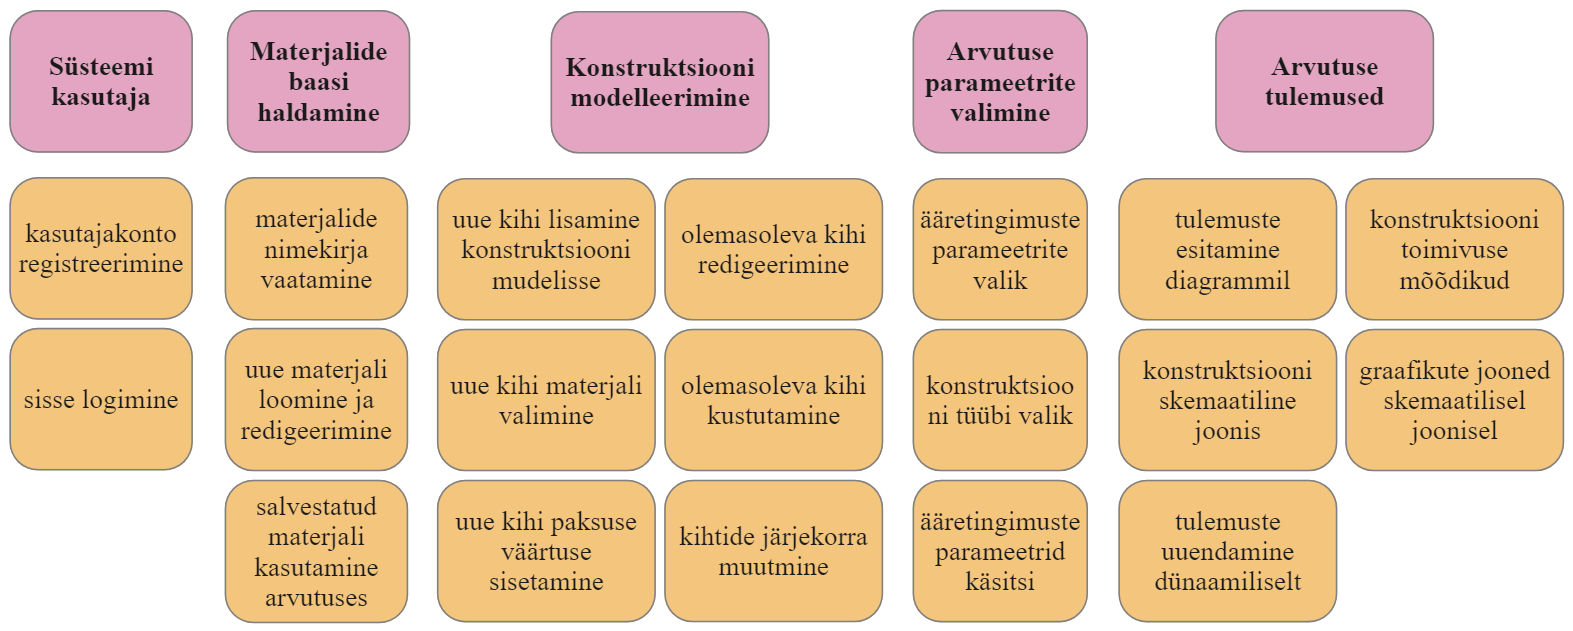
\includegraphics[width=1\textwidth]{figures/analysis/client_userstories0.png}
    \caption[Funktsionaalsed nõuded, kliendi kasutajalood]{\textit{Kliendi kasutajalood}}
    \label{fig:client_userstories}
\end{figure}


\subsection{Mittefunktsionaalsed nõuded}
Lisaks osas \ref{subsec_func_req} kirjeldatud funktsionaalsetele nõuetele, peab süsteem vastama järgmistele nõuetele:
\begin{itemize}
    \item kasutajaliides peab olema kiire -- kasutaja peab nägema arvutuse tulemuste uuendamist kohe peale 
lähteandmete (kihid, parameetrid) muutmist, pikk ooteaeg või lehe ümberlaadimine tulemuste näitamiseks ei ole aktsepteeritav;
    \item kasutajaliides peab olema kasutajasõbralik -- kasutaja peab intuitiivselt aru saama, mida ta peaks tegema, et 
jõuda tulemuseni, vajadusel peab ta olema juhitud \textit{popup}-tüüpi infoplokidega;
    \item kasutajaliides peab olema kaasaaegne, st välimus ja veebilehe struktuur peavad
vastama kaasaaegsetele UX/UI printsiipidele.
\end{itemize}
